\documentclass[a4paper, 10pt, dvipdfmx]{jlreq}

\usepackage{amsmath,amsfonts,amssymb}
\usepackage{bm}
\usepackage{mathtools}
\usepackage{siunitx}
\usepackage[dvipdfmx]{graphicx}
\usepackage[dvipdfmx]{color}
\usepackage[dvipdfmx, colorlinks=true, allcolors=blue]{hyperref}
\usepackage{listings, jlisting}
\usepackage{tikz}
\usepackage{physics}
\usepackage{url}

\Urlmuskip=0mu plus 10mu
\allowdisplaybreaks[4]
\frenchspacing
\definecolor{OliveGreen}{rgb}{0.0,0.6,0.0}
\definecolor{Orenge}{rgb}{0.89,0.55,0}
\definecolor{SkyBlue}{rgb}{0.28, 0.28, 0.95}
\lstset{
  language={c++},
  basicstyle={\ttfamily},
  identifierstyle={\small},
  ndkeywordstyle={\small},
  frame=single,
  breaklines=true,
  numbers=left,
  xrightmargin=0zw,
  xleftmargin=3zw,
  numberstyle={\scriptsize},
  lineskip=-0.9ex,
  keywordstyle={\small\bfseries\color{SkyBlue}},  
  commentstyle={\color{OliveGreen}}, 
  stringstyle={\small\ttfamily\color{Orenge}}    
}

\begin{document}

\title{2015年度 大問3}
\author{hari64boli64 (hari64boli64@gmail.com)}
\date{\today}
\maketitle

\section{問題}

\section{解答}

% \subsection*{(1)}

\begin{figure}[htbp]
  \begin{center}
    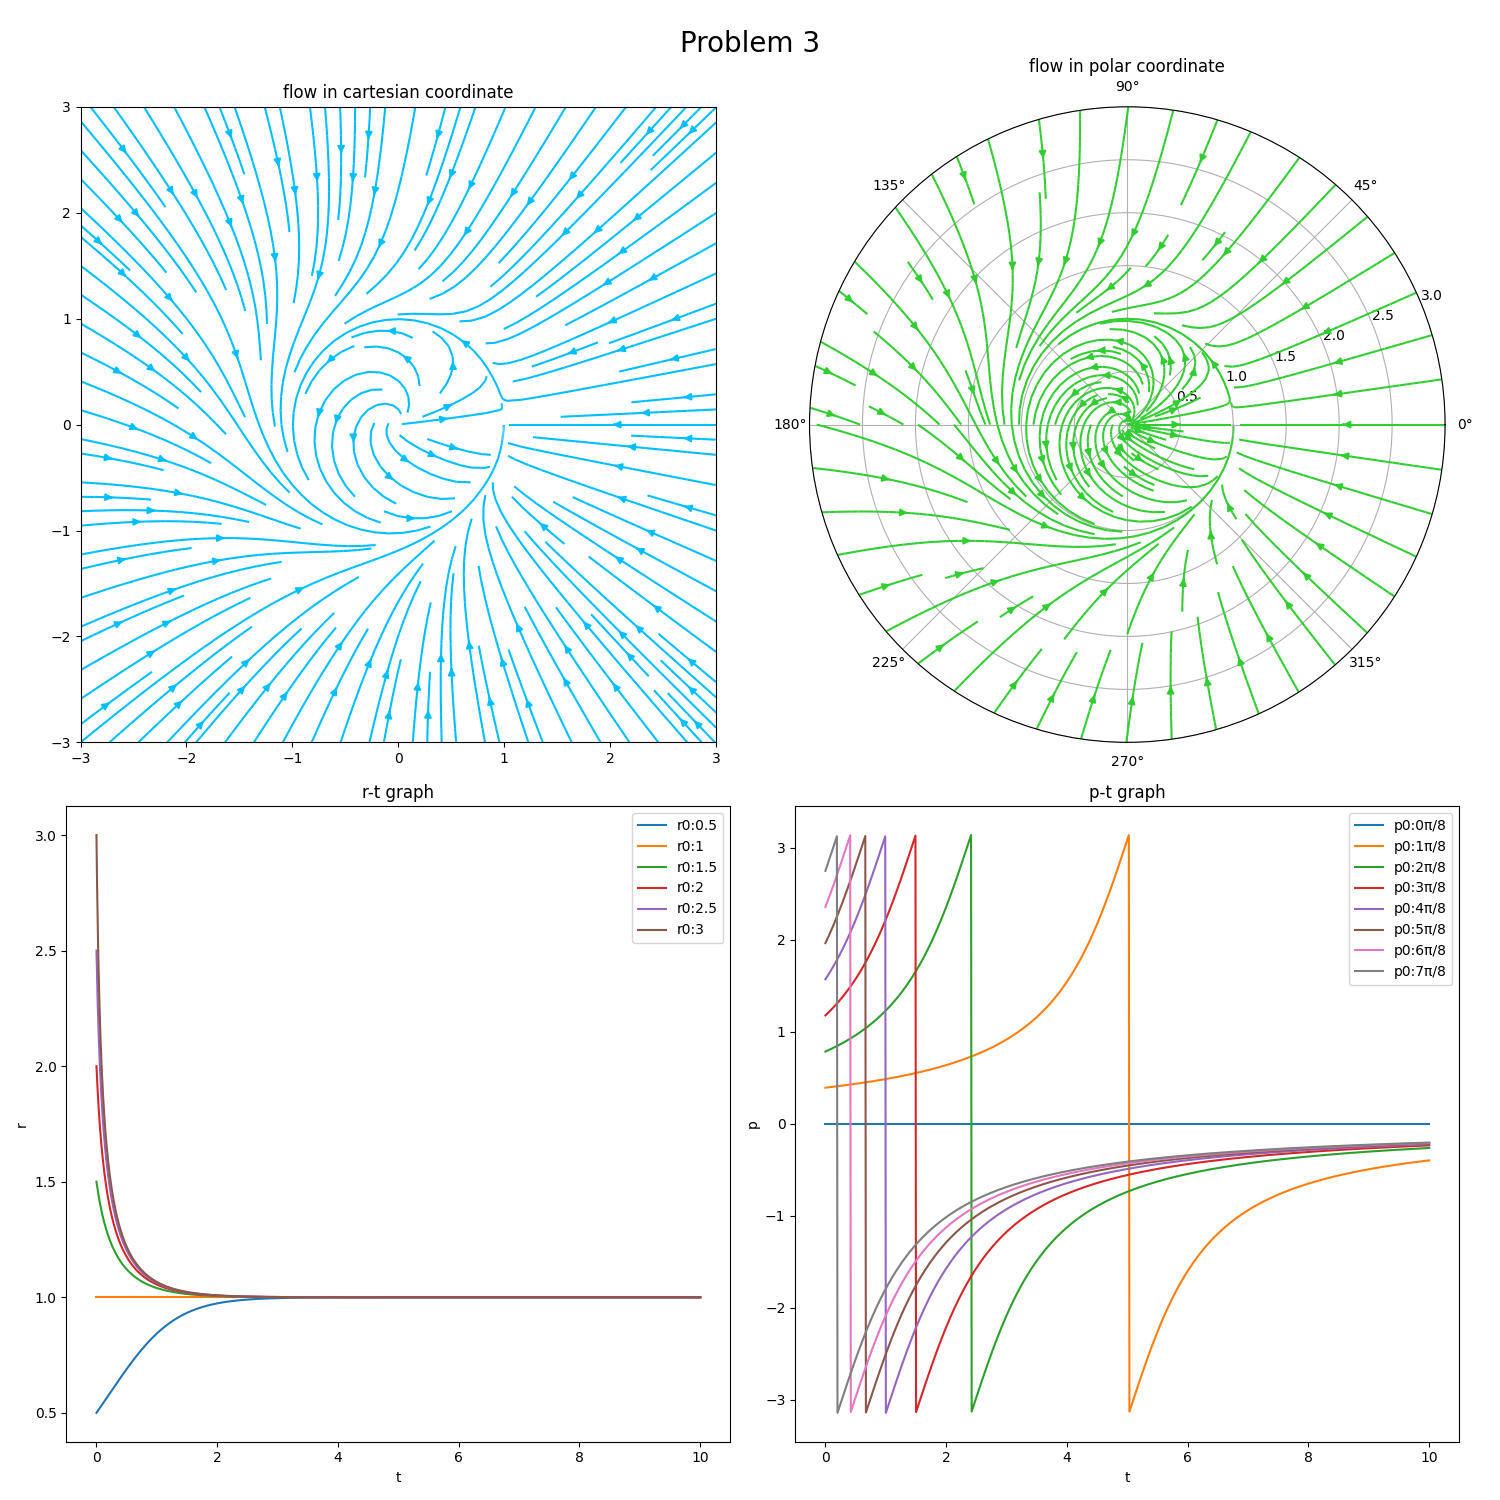
\includegraphics[height=120mm]{3.png}
    \caption{visualizations}
    \label{img:vis}
  \end{center}
\end{figure}

\section{知識}

\section{おまけ}

\lstinputlisting[caption=visualizer,label=code:visualizer,language=Python]{3.py}

\begin{thebibliography}{9}
  matplotlib.“matplotlib.pyplot.streamplot”.2020年1月5日.\url{https://matplotlib.org/3.1.1/api/_as_gen/matplotlib.pyplot.streamplot.html}
\end{thebibliography}

\end{document}
